\section{An\'alisis sint\'actico}

El an\'alisis sint\'actico es un an\'alisis a nivel de sentencias, y es mucho m\'as complejo que el an\'aisis l\'exico. Su funci\'on es tomar el programa fuente en forma de tokens, que recibe del analizador l\'exico, y determinar la estructura de las sentencias del programa. Este proceso es similar a determinar la estructura de una frase, determinando quien es el sujeto, predicado, el verbo y los complementos.

El an\'alisis sint\'actico agrupa a los tokens en clases sint\'acticas (denominadas no terminales en la definici\'on de la gram\'atica), tales como expresiones, procedimientos, etc.
El analizador sint\'actico o parser obtiene un \'arbol sint\'actico (u otra estructura equivalente) en la cual las hojas son los tokens, y cualquier nodo que no sea una hoja, representa un tipo de clase sint\'actica (operaciones).

Los \'arboles sint\'acticos se construyen con un conjunto de reglas conocidas como gram\'atica, y que definen con total precisi\'on el lenguaje fuente.

Al proceso de reconocer la estructura del lenguaje fuente se conoce con el nombre de an\'alisis sint\'actico (parsing). Hay distintas clases de analizadores o reconocedores sint\'acticos, pero en general se clasifican en 2 grandes grupos: A.S. Ascendentes y A.S. Descendentes.

La principal tarea del analizador sint\'actico no es comprobar que la sintaxis del programa fuente sea correcta, sino construir una representaci\'on interna de ese programa y en el caso en que sea un programa incorrecto, dar un mensaje de error.

Para ello, el analizador sint\'actico (A.S.) comprueba que el orden en que el analizador l\'exico le va entregando los tokens es v\'alido. Si esto es as\'i significar\'a que la sucesi\'on de s\'imbolos que representan dichos tokens puede ser generada por
la gram\'atica correspondiente al lenguaje del c\'odigo fuente. \cite{sintac}

	\begin{figure}[htbp!]
		\centering
			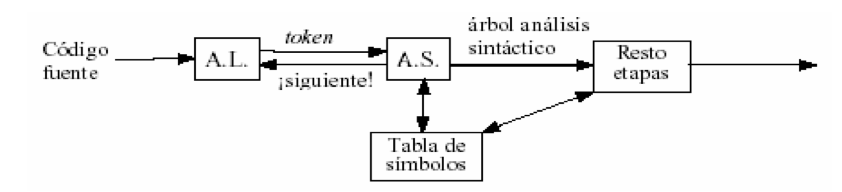
\includegraphics[width=0.8\textwidth]{images/analizadorS}
		\caption{An\'alisis sint\'actico.}
	\end{figure}
	
	\pagebreak
	
	%http://www.udb.edu.sv/udb/archivo/guia/informatica-ingenieria/compiladores/2013/ii/guia-3.pdf